\documentclass{article}
\usepackage{graphicx}
\usepackage[margin=1in]{geometry}
\begin{document}
\section{Problem 1}
\section{Pressure Drop Quantification}
See the appendix for the unabridged calculations associated with the following results.

The force imparted by the turbine on the wind can be solved for using conservation of momentum in integral form:

\begin{equation}
\frac{\partial}{\partial t} \int_{CV} \rho \underline{u} dV + \int_{CS} \rho (\underline{u} \cdot \hat{n} dA = \underline{f},
\end{equation}
where t is time, CV is the control volume, $\rho$ is the density of air, $\underline{u}$ is the velocity vector, CS is the control surface, $\hat{n}$ is the unit vector normal to the control surface, and $\underline{f}$ is the external force caused by the turbine.

For any streamtube of air flowing pas a turbine, conservation of mass may be applied to show that

\begin{equation}
A_W U_W = A_\infty U_\infty = A_D U_D,
\end{equation}
Where $A_W$ is the downstream area of the streamtube, $U_W$ is the downstream velocity of the streamtube, $A_\infty$ is the upstream area of the streamtube, $U_\infty$ is the upstream velocity of the streamtube (i.e., the inflow velocity), $A_D$ is the diameter of the turbine, and $U_D$ is the velocity of the air before it passes through the turbine.

These equations may be applied to the left and right sides of the turbine separately, assuming a steady flow, to obtain the following relation:

\begin{equation}
f_x = u_\infty (1-a)A_D\rho (u_infty - u_w).
\end{equation}

It may be observed that the force imparted by the turbine on the wind is equal and opposite to the force the wind exerts on the turbine:

\begin{equation}
f_x = (P_D^+ - P_D^-)A_D = u_\infty (1-a)A_D\rho (u_infty - u_w).
\end{equation}

\subsection{The Wake Magnitude's Relationship to Inflow Speed and Axial Induction Factor}
\subsection{Relationship Between Power Production and Axial Induction Factor}
\section{Problem 2}
The PARK wake model was used to model the 
wind speed profile of an array of ten turbines, spaced 400 meters apart and aligned in the streamwise direction. This power plant does not optimize its power production when each turbine is operating to maximize its individual energy captured. The axial induction factors were optimized using the Nelder-Mead simplex optimization algorithm. The power production and velocity incoming to each turbine are show in Figure \ref{p1} for the baseline case where each axial induction factor is $\frac{1}{3}$, and using the optimized axial induction factors. 

\begin{figure}[htb!]
\centering
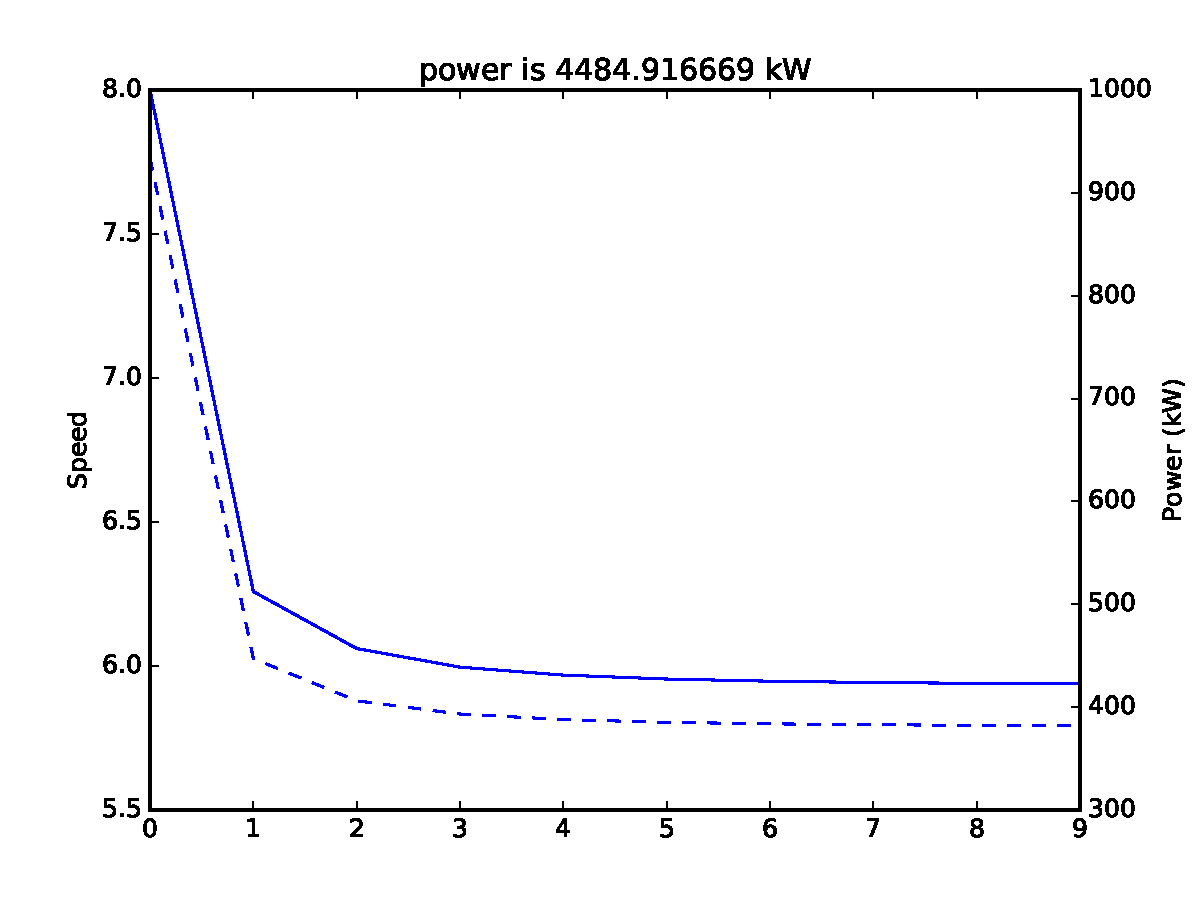
\includegraphics[scale=.3]{speed}
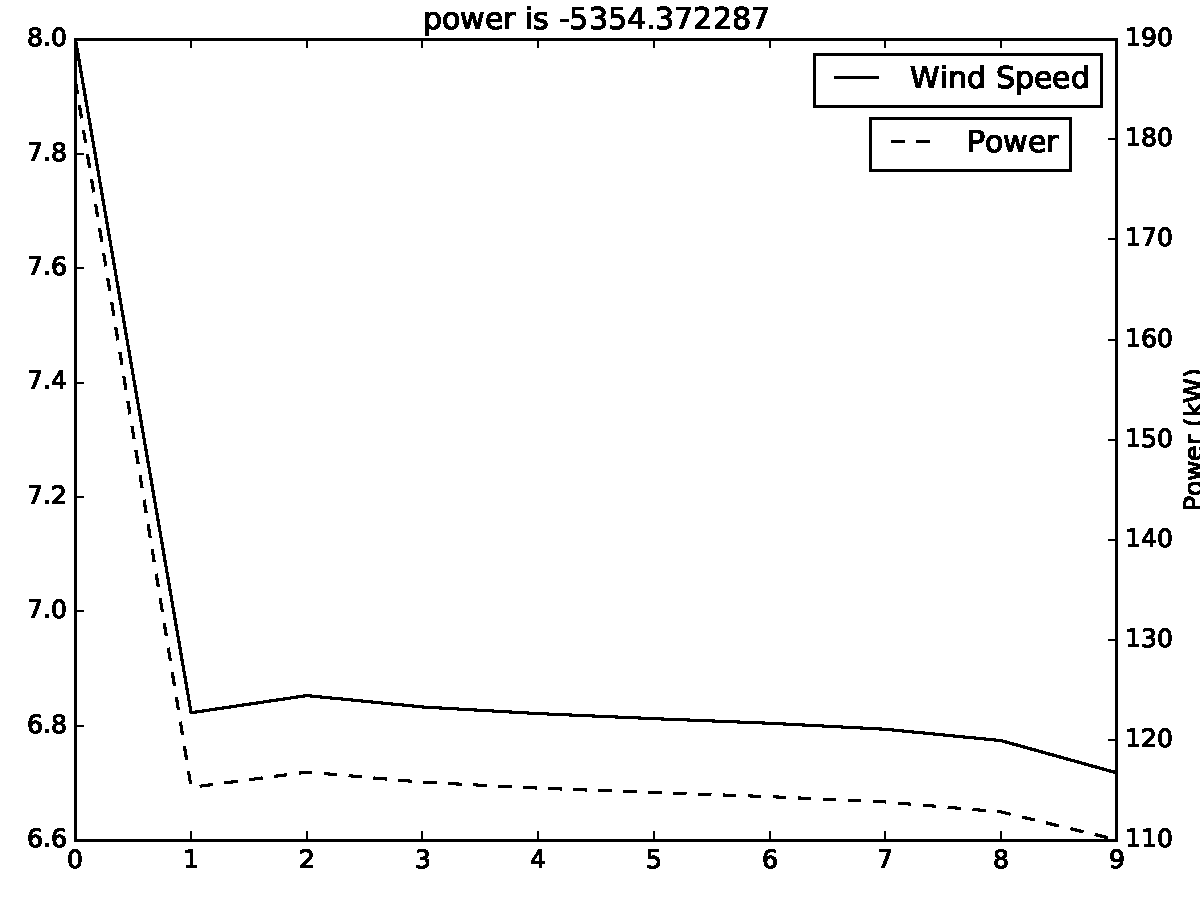
\includegraphics[scale=.3]{optimized}
\caption{\label{p1} Power production and velocity profile for (left) baseline axial induction settings and (right) optimized axial induction settings}
\end{figure}

\section{Problem 3}
Wake models were developed using ideal flow theory and a point-source boundary layer wake model. Both of these models model the turbine wake in two dimensions, neglecting the vertical dimension. The minimum spacing between turbines to achieve 99\% reduction in the velocity deficit is reported for both models.

\subsection{Ideal Flow Wake Model}
An ideal flow wake model was constructed using point sources and sinks and a uniform inflow. The sources and sinks were placed in an alternating fashion along the 80 meter turbine rotor diameter. The stream function used was

\begin{equation}
\psi = U y + \sum_{t=1}^T \sum_n^N (-1)^n m \arctan\left( (y + (n-40) \frac{80}{N}, (x - x_t)\right) 
\end{equation}

Contours of $\psi$ represent the flow streamlines. The flow field associated with one turbine is shown in Figure XX. The streamlines streamlines stabilize 1500 meters downstream of the turbine, indicating that this is where the velocity deficit caused by the upstream turbine would be negligible.

\begin{figure}[htb!]
\centering
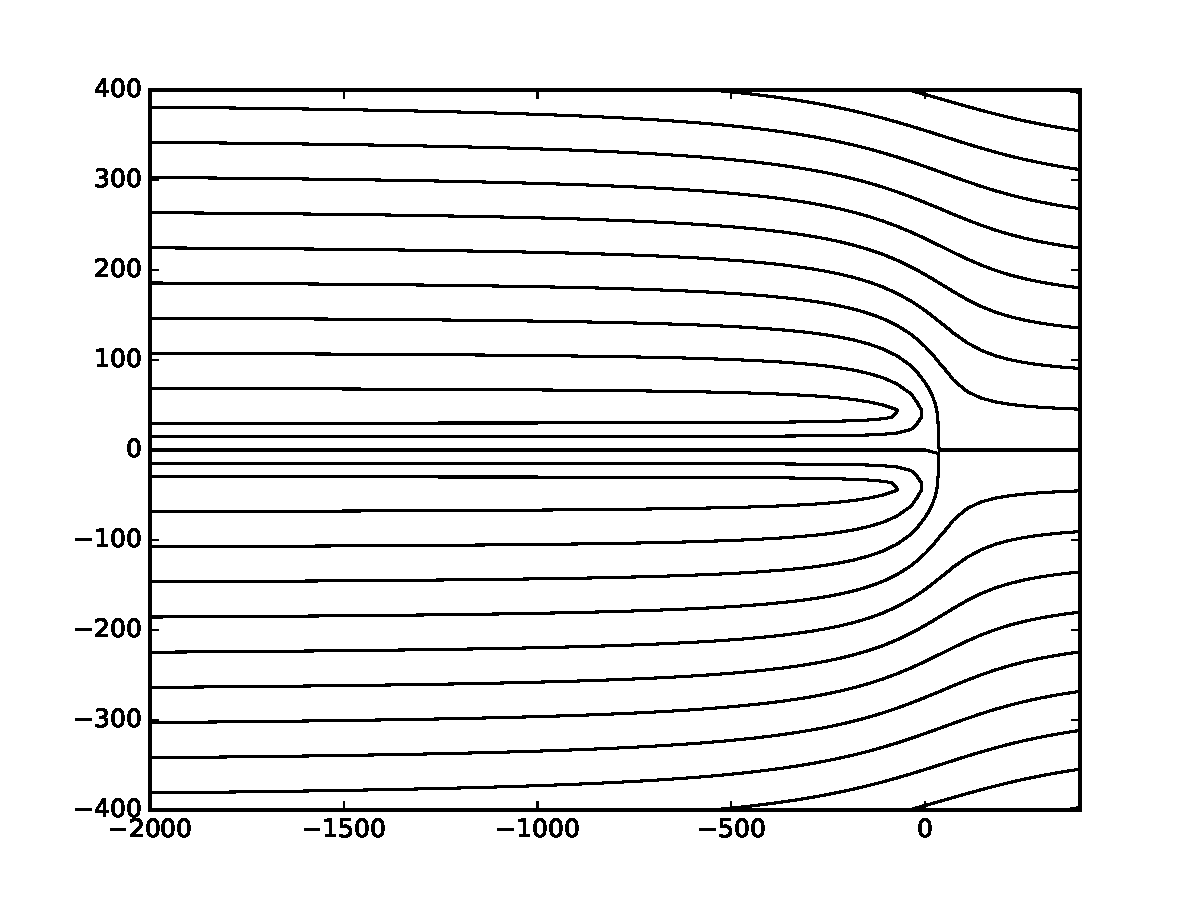
\includegraphics[scale=.4]{oneturb}
\caption{\label{oneturb} Flow field associated with ideal flow wake model for one turbine. The flow moves from right to left.}
\end{figure}

In the case of two turbines (one directly waking the other), the required spacing for the streamlines to stabilize was found to be 2500 meters, indicating that is the required spacing for the velocity deficit for the upstream turbine to be minimal. The flow field associated with this spacing is shown in Figure \ref{twoturbs}

\begin{figure}[htb!]
\centering
\includegraphics[scale=.4]{twoturbs}
\caption{\label{twoturbs} Flow field associated with ideal flow wake model for two turbines spaced 2500 meters apart. The flow moves from right to left.}
\end{figure}

\subsection{Point-Source Boundary Layer Model}
The second turbine wake model developed was a point-source boundary layer wake model. A point source origin was modeled as being located far away to give the velocity profile a width that is realistic for an 80 meter diameter turbine. The point-source boundary layer velocity deficit model used was

\begin{equation}
u_{deficit} = \frac{D}{\rho(4 \pi u_0 \nu)^2} \left(x-x_0\right)^{-\frac{1}{2}} \exp{\left(\frac{-u_0 y ^2}{4\nu (x-x_0)}\right)}
\end{equation}
where $u_{deficit}$ is the velocity deficit predicted by the wake model, D is the momentum flux produced by the turbine, $\rho$ is the air density (1.225 $\frac{kg}{m^3}$, $\nu$ is the kinematic viscosity ($15.11x10^{-5} \frac{m^2}{s}$, $x$ and $y$ are the streamwise and crossflow positions in the flow field, $x_0$ is the origin of the point-source wake, and $u_0$ is the upstream wind speed (8 m/s).

The wake model is shown for a single turbine in Figure \ref{blw}. The wake decays slowly, requiring around 600,000,000 meters for the deficit to reach 1\% of the upstream wind speed.

\begin{figure}[htb!]
\centering
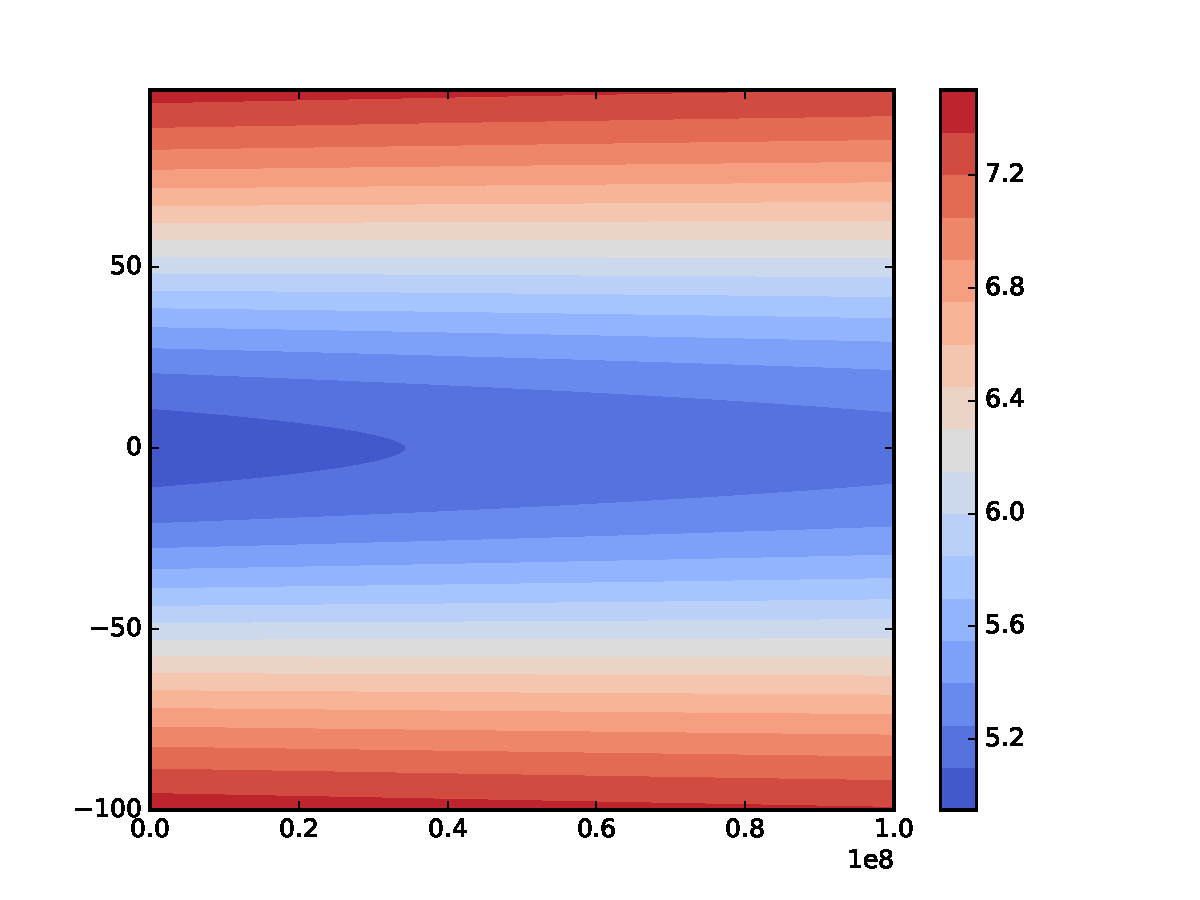
\includegraphics[scale=.5]{boundarywake}
\caption{\label{blw}Point-source boundary layer wake model}
\end{figure}

The velocity deficit shows exponential decay. We plot the centerline velocity profile in Figure \ref{p3cl}. I expected the wake to decay with a much slower rate. The wake decays with a $\frac{1}{\sqrt{x}}$ relationship, so I expected a 1\% decay to be associated with $\frac{1}{0.01^2}$, which is 1,000 meters.

\begin{figure}[htb!]
\centering
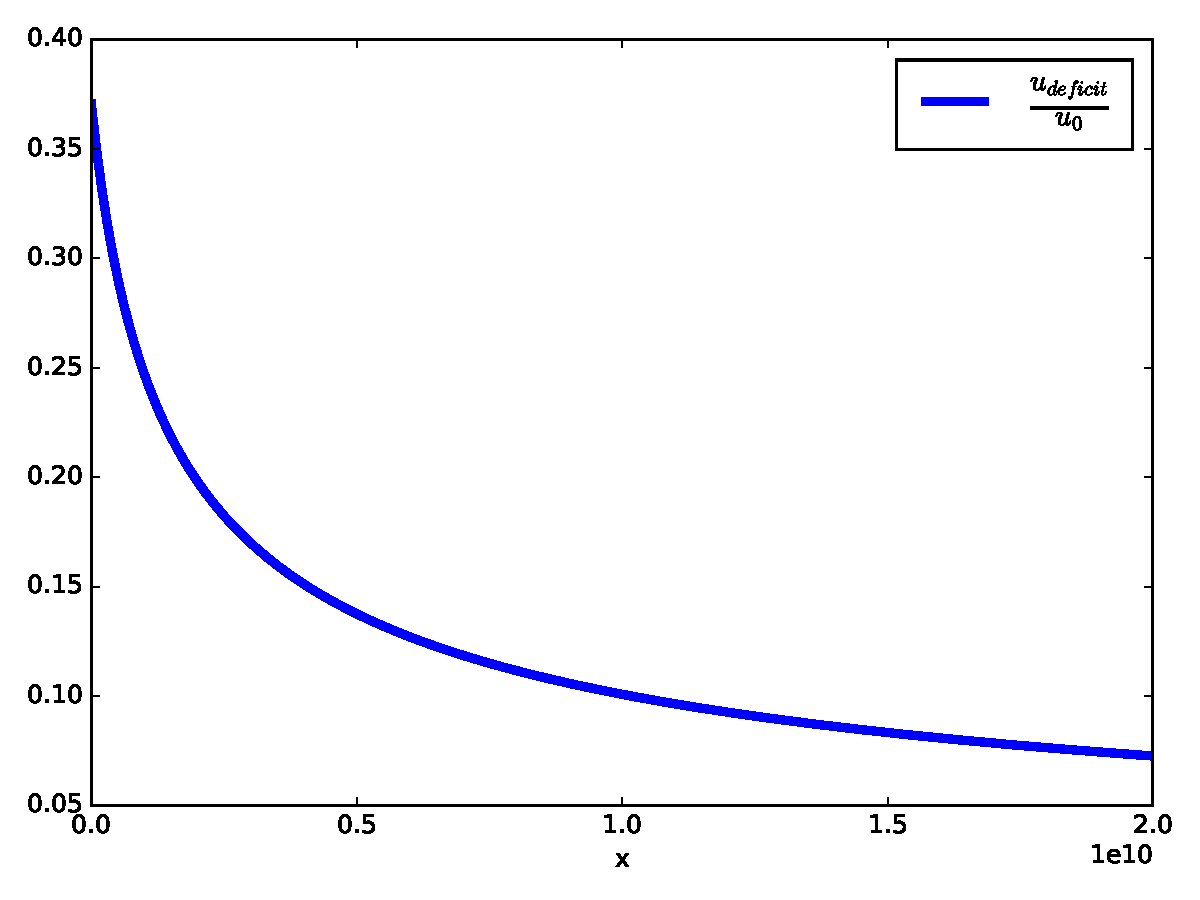
\includegraphics[scale=.5]{p3centerline}
\caption{\label{p3cl} Centerline velocity profile of the boundary layer wake model}
\end{figure}

\begin{figure}[htb!]
\centering
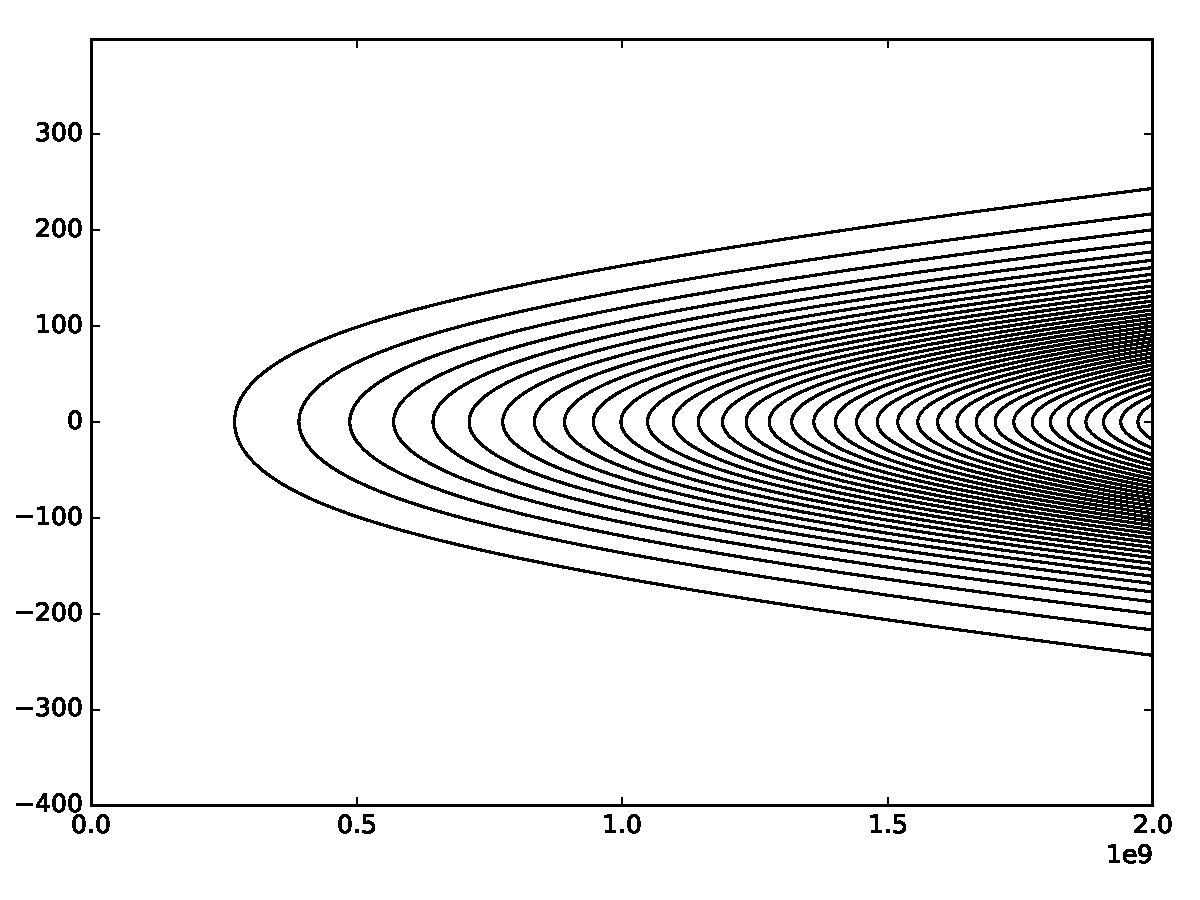
\includegraphics[scale=.6]{p3streams}
\caption{\label{p3streams}The flow moves from left to right.}
\end{figure}

TODO two turbs

\section{Problem 4}
I implemented the PARK wake model. The velocity deficit imparted on a flow field by a wind turbine is described as
\begin{equation}
U_{def} = \frac{U_0 2a}{( 1 + \frac{ 2 k \Delta x}{D}) ^ 2}
\end{equation}
where $U_0$ is the velocity incoming to the turbine, k is the wake expansion coefficeint, $\Delta X$ is the distance downstream of the turbine, and this deficit is applied where $y_0 - \frac{D}{2} - kx < y <  y_0 + \frac{D}{2} + kx$, where $y_0$ is the location of the turbine in the cross-flow direction.

Three  turbine layouts were used to gain intuition for the model: a uniform grid, a circular layout, and placing the turbines at the inflow and outflow boundaries.

\begin{figure}[htb!]
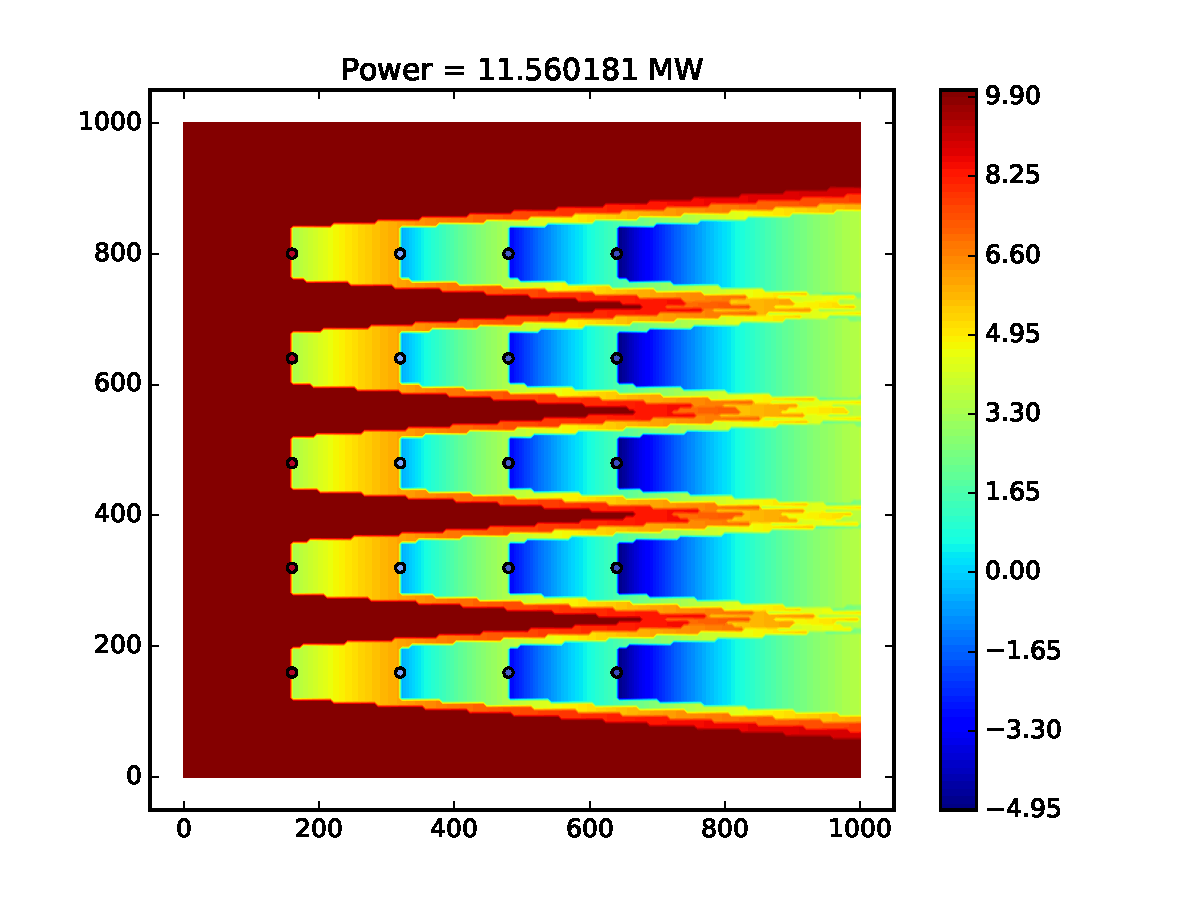
\includegraphics[scale=.25]{grid}
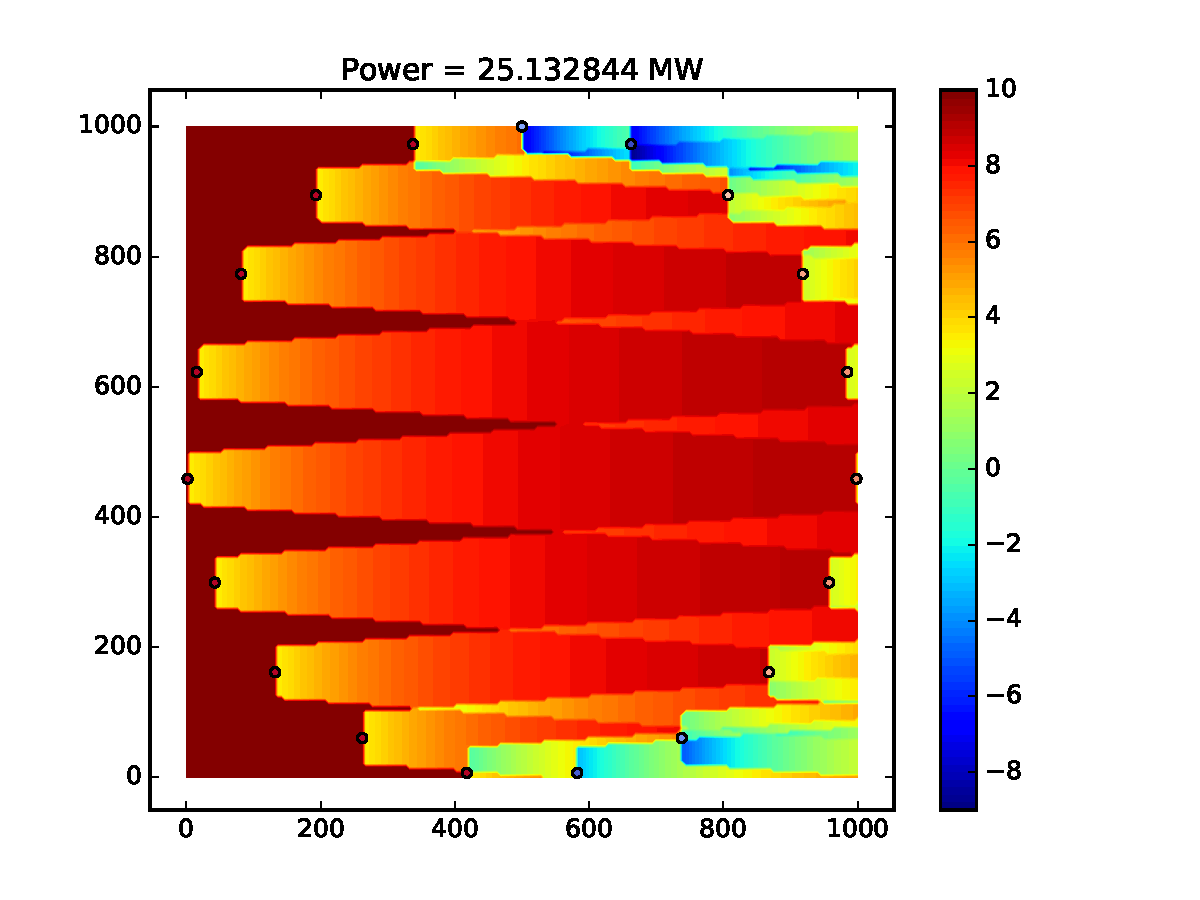
\includegraphics[scale=.25]{circle}
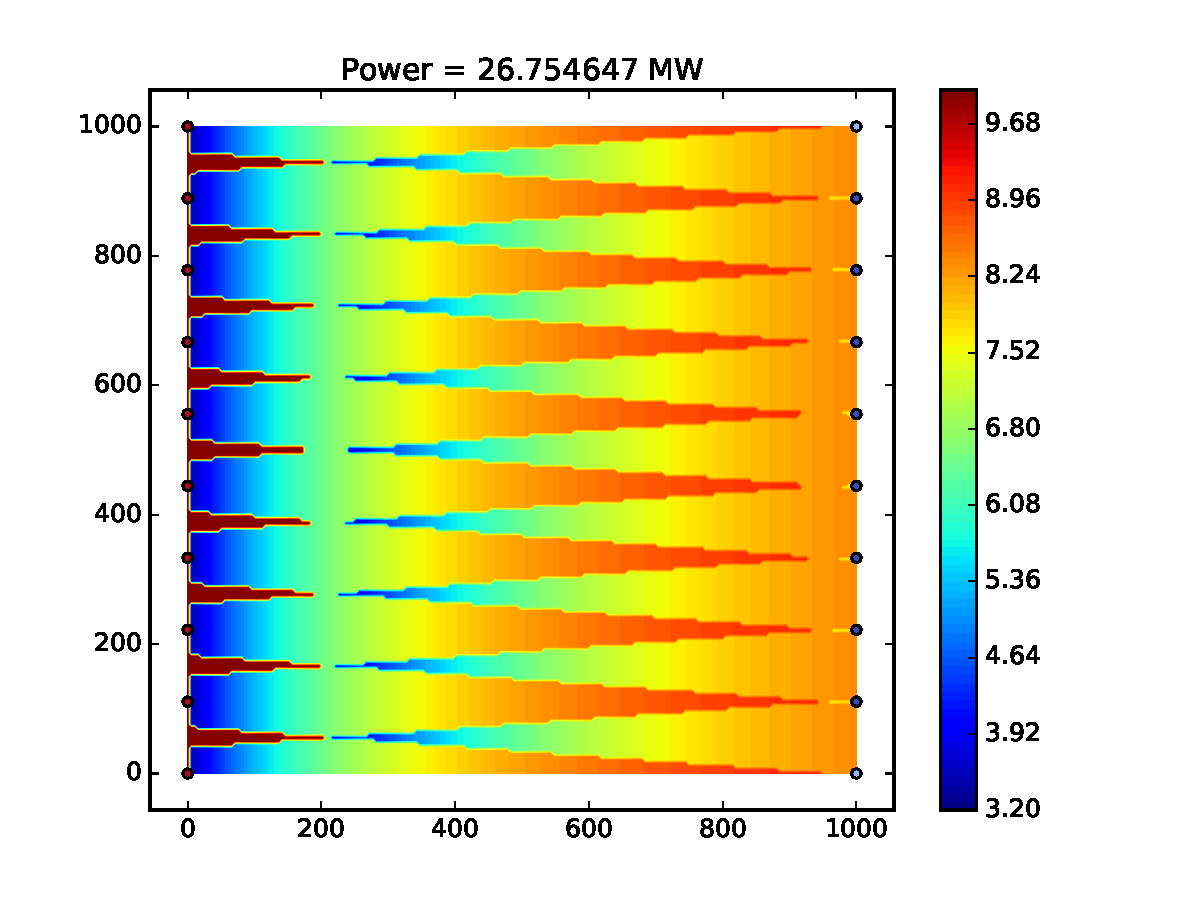
\includegraphics[scale=.25]{edges}
\end{figure}

Optimization was performed of the turbines' layout and axial induction factors. The positions were optimized first and the axial induction factors were then optimized. It is likely that even better power porduction could be achieved by coupling these optimization schemes.

The layout was optimized using the Constrained Optimization by Linear Approximation algorithm. Several constraints were applied for the spacing between each pair of turbines. A multistart approach was used, randomly initializing the turbine positions and selecting the first solution that did not violate the spacing constraints.

\begin{figure}[htb!]
\centering
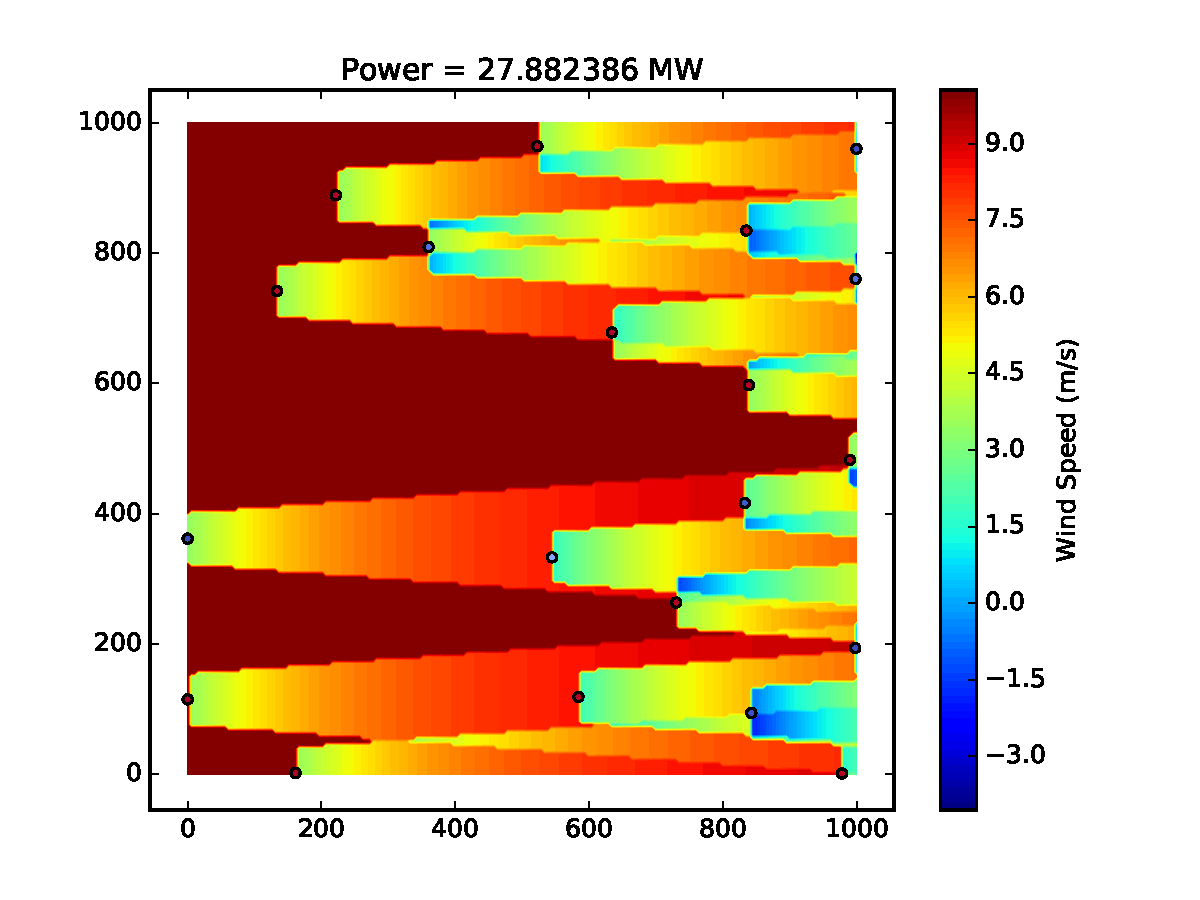
\includegraphics[scale=.6]{optlayout1}
\caption{\label{opt} OPtimized wind turbine layout}
\end{figure}

\end{document}